\documentclass[aspectratio=169,12pt]{beamer}

\usetheme{Madrid}
\usecolortheme{seahorse}
\setbeamertemplate{navigation symbols}{}
\setbeamertemplate{footline}[frame number]

\usepackage{amsmath,amssymb}
\usepackage{graphicx}
\usepackage{xcolor}
\usepackage{tikz}
\usetikzlibrary{arrows.meta,positioning}
\usepackage{listings}

\graphicspath{{../../plots/}}

\definecolor{topological}{HTML}{1f77b4}
\definecolor{critical}{HTML}{2ca02c}
\definecolor{trivial}{HTML}{d62728}
\definecolor{edgemode}{HTML}{e377c2}
\definecolor{codebg}{HTML}{f5f5f5}
\definecolor{codekw}{HTML}{0000cd}
\definecolor{codecomment}{HTML}{228b22}

\lstset{
  language=Python,
  basicstyle=\ttfamily\scriptsize,
  keywordstyle=\color{codekw}\bfseries,
  commentstyle=\color{codecomment}\itshape,
  backgroundcolor=\color{codebg},
  frame=single,
  showstringspaces=false,
  breaklines=true
}

\newcommand{\ket}[1]{|#1\rangle}
\newcommand{\Oedge}{X_0Z_1\cdots Z_{L-2}X_{L-1}}

\title[Kitaev Chain -- Block 3]{Majorana Modes in the Machine}
\subtitle{Week 7: From ED Validation to a Real VQE Sweep}
\author{Dobromir Stoev\\ Edgar Harutyunyan\\ Guilherme Schewtschik\\ Jaskaran Singh\\ Zhengyi Liu\\ Zhenming Shi}
\institute{Advanced Seminar -- AI-Augmented Theoretical Physics}
\date{\today}

\begin{document}

\begin{frame}
  \titlepage
\end{frame}

\begin{frame}{Week 7 Objective}
  \begin{block}{Milestone}
    Replace the exact-diagonalization state preparation used in Week 6 with a parity-constrained VQE preparation at every point of the $\mu$ sweep.
  \end{block}

  \begin{itemize}
    \item Keep the same Hamiltonian, edge-string observable, and shot-measurement protocol.
    \item Reuse the existing $L=4$ hardware-efficient ansatz and optimizer workflow.
    \item Validate every VQE state against ED before introducing hardware noise.
    \item Produce a VQE-prepared phase sweep that can become the noiseless Block 4 baseline.
  \end{itemize}
\end{frame}

\begin{frame}{Where Week 6 Stops}
  \begin{columns}[T]
    \begin{column}{0.64\textwidth}
      \centering
      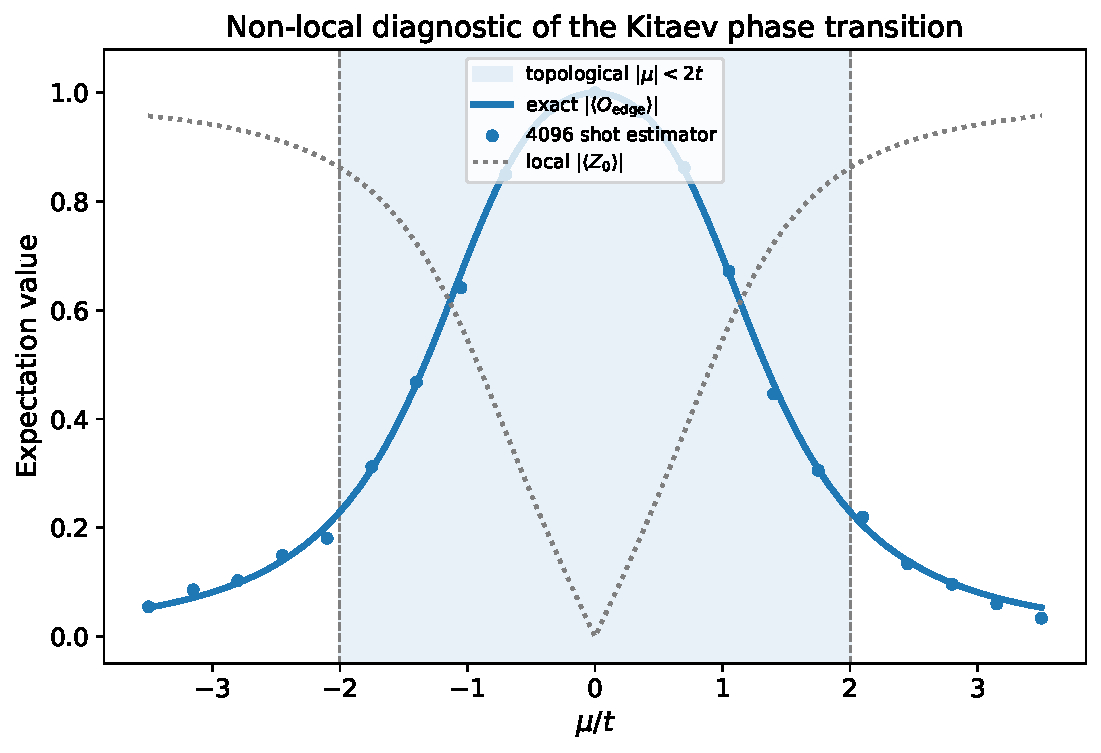
\includegraphics[width=\textwidth]{block3_week6_phase_sweep.pdf}
    \end{column}
    \begin{column}{0.33\textwidth}
      \small
      \textbf{Already established}
      \begin{itemize}
        \item Sweep target: $\langle\Oedge\rangle$
        \item ED parity-gap cross-check
        \item Synthetic shot estimator
      \end{itemize}
      \textbf{Remaining gap}
      \begin{itemize}
        \item Every plotted state is prepared by ED, not VQE.
      \end{itemize}
    \end{column}
  \end{columns}
\end{frame}

\begin{frame}{Existing VQE Baseline}
  \begin{columns}[T]
    \begin{column}{0.60\textwidth}
      \centering
      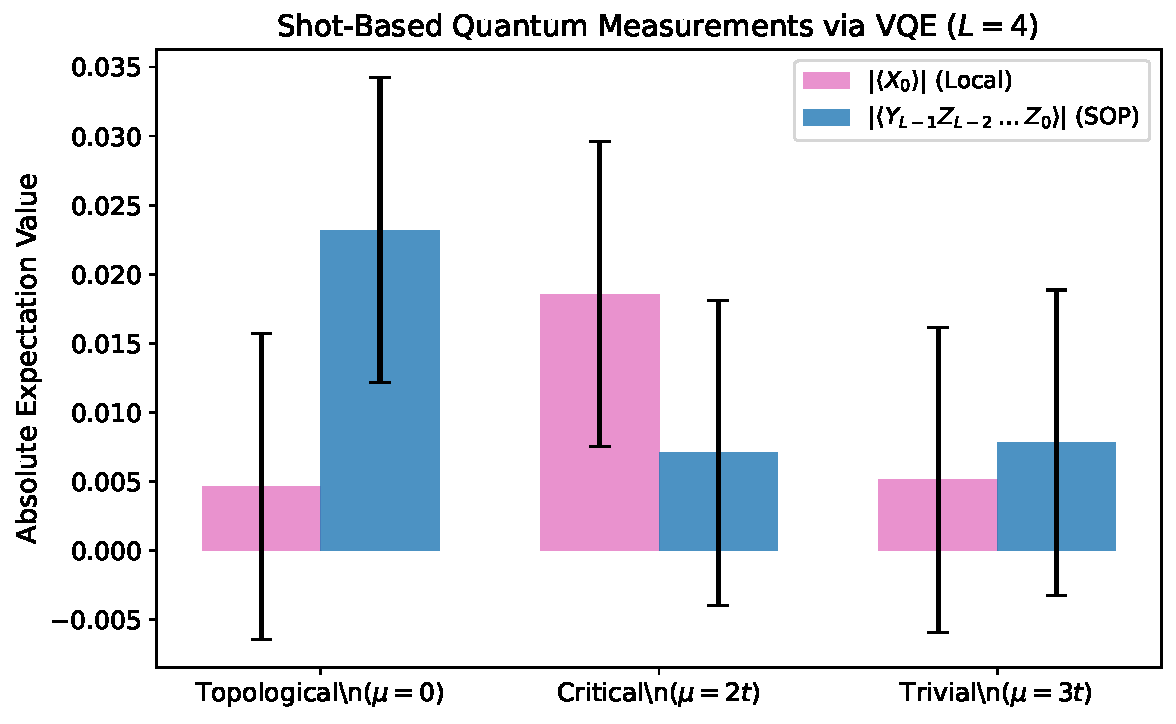
\includegraphics[width=\textwidth,height=0.66\textheight,keepaspectratio]{block3_01_vqe_observables_test.pdf}
    \end{column}
    \begin{column}{0.36\textwidth}
      \small
      Existing components:
      \begin{itemize}
        \item \texttt{EfficientSU2}: $R_Y$ + linear CNOTs
        \item Aer estimator + multi-start COBYLA
        \item ED fidelity checks
        \item Shot measurements
      \end{itemize}
      Current scope: three representative $\mu$ values.
    \end{column}
  \end{columns}
\end{frame}

\begin{frame}{The VQE Sweep Workflow}
  \centering
  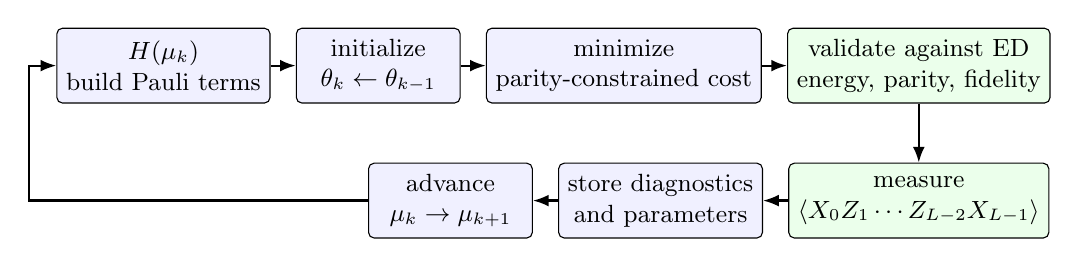
\begin{tikzpicture}[
    node distance=0.42cm and 0.32cm,
    box/.style={draw,rounded corners=2pt,align=center,minimum height=0.95cm,minimum width=2.08cm,fill=blue!6,font=\small},
    check/.style={box,fill=green!8},
    arrow/.style={-{Latex[length=2mm]},thick}
  ]
    \node[box] (ham) {$H(\mu_k)$\\build Pauli terms};
    \node[box,right=of ham] (init) {initialize\\$\theta_k\leftarrow\theta_{k-1}$};
    \node[box,right=of init] (opt) {minimize\\parity-constrained cost};
    \node[check,right=of opt] (validate) {validate against ED\\energy, parity, fidelity};
    \node[check,below=0.75cm of validate] (measure) {measure\\$\langle\Oedge\rangle$};
    \node[box,left=of measure] (store) {store diagnostics\\and parameters};
    \node[box,left=of store] (next) {advance\\$\mu_k\rightarrow\mu_{k+1}$};
    \draw[arrow] (ham)--(init);
    \draw[arrow] (init)--(opt);
    \draw[arrow] (opt)--(validate);
    \draw[arrow] (validate)--(measure);
    \draw[arrow] (measure)--(store);
    \draw[arrow] (store)--(next);
    \draw[arrow] (next.west) -| ([xshift=-0.35cm]ham.west) |- (ham.west);
  \end{tikzpicture}

  \vspace{0.35cm}
  \begin{block}{Key engineering change}
    The optimizer is no longer restarted independently at every $\mu$; neighboring ground states seed one another.
  \end{block}
\end{frame}

\begin{frame}{Why Warm Starts Matter}
  \begin{columns}[T]
    \begin{column}{0.48\textwidth}
      \textbf{Independent random starts}
      \begin{itemize}
        \item Repeats expensive optimization work
        \item Can converge to different local minima
        \item Makes the sweep noisy even before shot noise
      \end{itemize}
    \end{column}
    \begin{column}{0.48\textwidth}
      \textbf{Continuation in $\mu$}
      \begin{itemize}
        \item Use $\theta^*(\mu_k)$ to initialize $\mu_{k+1}$
        \item Exploits smooth ground-state evolution away from criticality
        \item Random restarts remain a fallback when validation fails
      \end{itemize}
    \end{column}
  \end{columns}

  \begin{alertblock}{Expected difficulty}
    Near $|\mu|=2t$, the bulk gap closes and the optimal state changes fastest; this is where warm starts and fidelity checks are most important.
  \end{alertblock}
\end{frame}

\begin{frame}{Parity Must Be Controlled}
  \begin{equation*}
    P=\prod_{j=0}^{L-1}Z_j,\qquad [H,P]=0
  \end{equation*}

  \begin{columns}[T]
    \begin{column}{0.48\textwidth}
      \textbf{Problem}
      \begin{itemize}
        \item The topological phase has nearly degenerate parity sectors.
        \item Energy minimization alone can return inconsistent sectors across the sweep.
        \item A sector jump can look like a discontinuity in the observable.
      \end{itemize}
    \end{column}
    \begin{column}{0.48\textwidth}
      \textbf{Week 7 strategy}
      \begin{equation*}
        C(\theta)=\langle H\rangle+\lambda\bigl(1-\langle P\rangle\bigr)^2
      \end{equation*}
      \begin{itemize}
        \item Target even parity consistently.
        \item Record $\langle P\rangle$ at every point.
        \item Reject states outside the parity tolerance.
      \end{itemize}
    \end{column}
  \end{columns}
\end{frame}

\begin{frame}{Validation Dashboard}
  \footnotesize
  A low VQE energy alone is not enough. Each point must pass four checks:

  \begin{center}
  \begin{tabular}{p{0.20\textwidth}p{0.31\textwidth}p{0.37\textwidth}}
    \textbf{Metric} & \textbf{Question} & \textbf{Use} \\
    \hline
    Energy error & Is $E_{\mathrm{VQE}}$ near $E_{\mathrm{ED}}$? & Detect optimizer failure \\
    Parity & Is $\langle P\rangle\approx+1$? & Keep one sector across $\mu$ \\
    Subspace fidelity & Does VQE overlap the correct low-energy space? & Handle near-degeneracy correctly \\
    String error & Matches the ED edge string? & Validate the quantity used in the phase sweep
  \end{tabular}
  \end{center}

  \begin{block}{Pass criterion}
    Failed points trigger deeper ansatz repetitions, additional optimizer iterations, or random-restart recovery.
  \end{block}
\end{frame}

\begin{frame}[fragile]{Implementation Shape}
\begin{lstlisting}
theta = initial_parameters()
for mu in mu_values:
    H = qiskit_hamiltonian(L, t, mu, delta)
    theta = optimize(parity_cost(H), initial=theta)

    diagnostics = validate(theta, H, ed_reference(mu))
    if not diagnostics.pass_all:
        theta = recover_with_restarts(H)

    string_value = measure_edge_string(theta, shots=4096)
    save(mu, theta, diagnostics, string_value)
\end{lstlisting}

\begin{itemize}\small
  \item The sweep must save optimizer parameters and diagnostics, not only the final observable.
  \item Reproducible checkpoints make failed regions debuggable and reusable for later noise studies.
\end{itemize}
\end{frame}

\begin{frame}{Week 7 Result: VQE-Prepared Sweep}
  \begin{columns}[T]
    \begin{column}{0.62\textwidth}
      \centering
      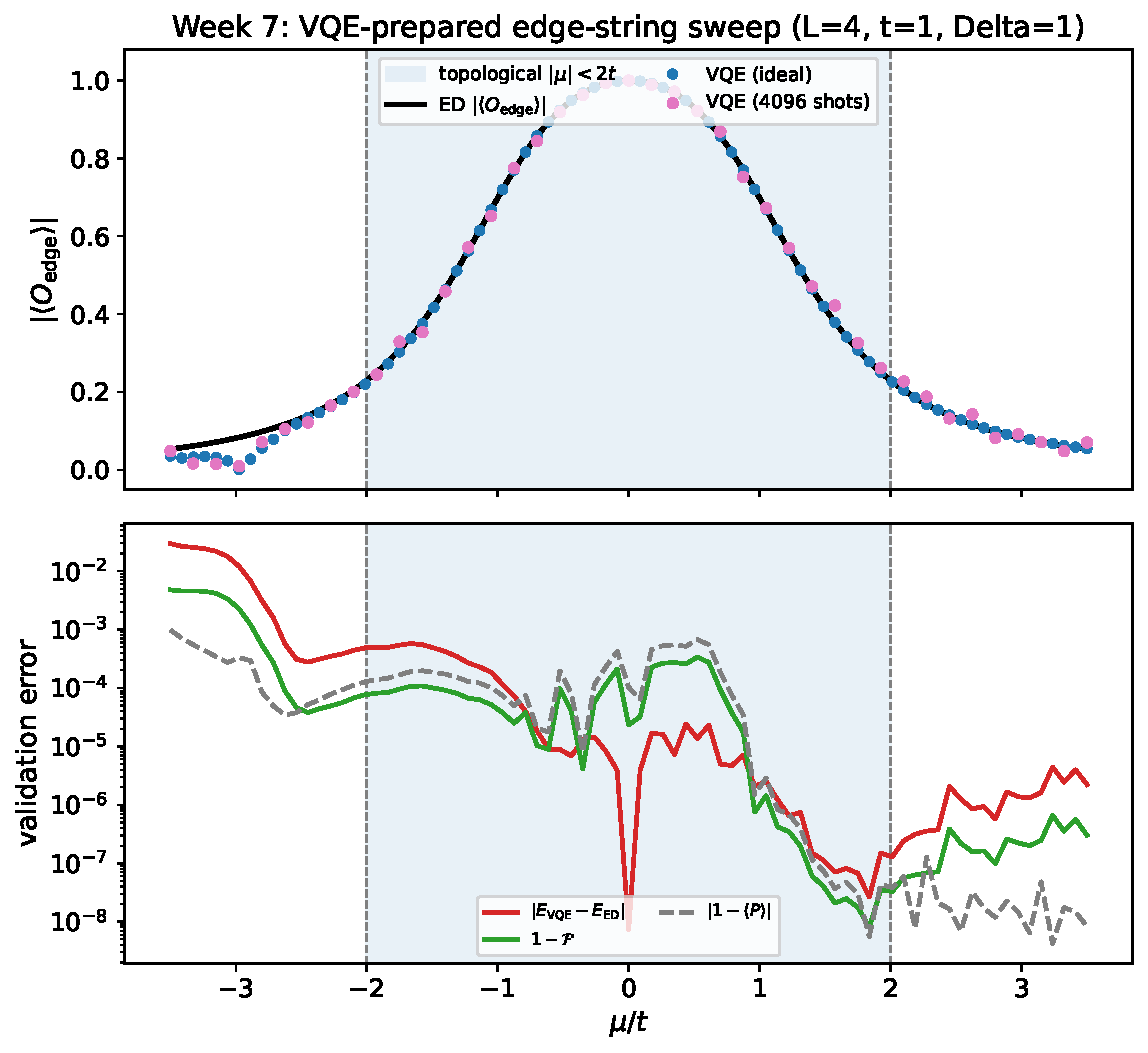
\includegraphics[width=\textwidth,height=0.82\textheight,keepaspectratio]{block3_week7_vqe_sweep.pdf}
    \end{column}
    \begin{column}{0.34\textwidth}
      \small
      \textbf{Top:} edge string $|\langle\Oedge\rangle|$ from parity-constrained VQE (ideal and shot-based) tracks the ED baseline across the whole $\mu$ grid.

      \vspace{0.25cm}
      \textbf{Bottom:} per-point validation --- energy error, infidelity $1-\mathcal{F}$, and parity deviation $|1-\langle P\rangle|$. Crosses mark points needing random-restart recovery.

      \vspace{0.25cm}
      Warm-start continuation keeps every point in the even sector.
    \end{column}
  \end{columns}
\end{frame}

\begin{frame}{Ansatz Depth: How Deep Is Enough?}
  \begin{columns}[T]
    \begin{column}{0.62\textwidth}
      \centering
      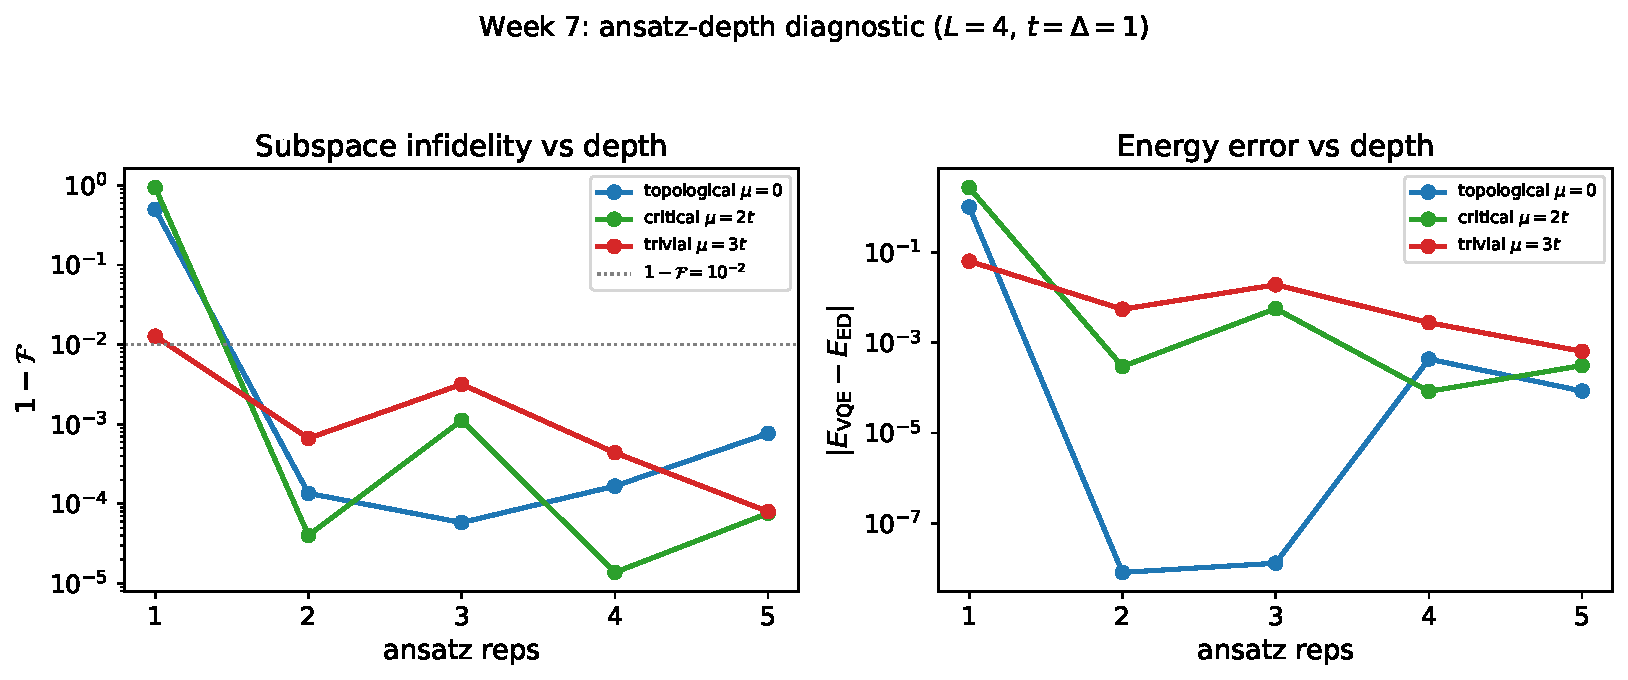
\includegraphics[width=\textwidth,height=0.78\textheight,keepaspectratio]{block3_week7_depth_fidelity.pdf}
    \end{column}
    \begin{column}{0.34\textwidth}
      \small
      Multi-start VQE at three representative $\mu$, scanning ansatz reps.
      \begin{itemize}
        \item $1$ rep ($8$ params) is too shallow, worst at $\mu=2t$ (fidelity $\sim 0.06$).
        \item $2$+ reps already reach the even-parity ground space.
        \item Criticality is the hardest point, exactly where the bulk gap closes.
      \end{itemize}
      This justifies the \texttt{reps}$=3$ used in the sweep.
    \end{column}
  \end{columns}
\end{frame}

\begin{frame}{Definition of Done for Week 7}
  \begin{itemize}
    \item A scripted $L=4$, $t=\Delta=1$ VQE sweep over the same $\mu$ grid as Week 6.
    \item Consistent even-parity preparation across the sweep.
    \item ED comparison for energy, parity, subspace fidelity, and edge-string expectation.
    \item Shot-based VQE edge-string curve plotted against the ED baseline.
    \item Optimization cost and failure/recovery statistics recorded per $\mu$ point.
  \end{itemize}

  \begin{block}{Boundary to Block 4}
    Only after the ideal VQE sweep passes validation should depolarizing, readout, and relaxation noise be added.
  \end{block}
\end{frame}

\begin{frame}{Next: Block 4 NISQ Reality Check}
  \begin{itemize}
    \item Freeze the validated ideal VQE sweep as the noiseless reference.
    \item Apply realistic gate, readout, and relaxation noise to preparation and measurement circuits.
    \item Separate optimizer degradation from measurement degradation.
    \item Compare raw and mitigated edge-string curves.
    \item Quantify when the inferred phase boundary becomes unreliable.
  \end{itemize}

  \begin{alertblock}{Conceptual progression}
    Week 6 validated the diagnostic with ED; Week 7 validates quantum state preparation; Block 4 tests whether the full workflow survives realistic noise.
  \end{alertblock}
\end{frame}

\end{document}
